\documentclass[12pt,english]{article}
\usepackage[T1]{fontenc}
\usepackage{amssymb,amsmath,amsthm}
\usepackage[table]{xcolor}
\usepackage{tikz}
\usetikzlibrary{shapes.geometric, fit,calc,positioning,decorations.pathreplacing,matrix, patterns}

\begin{document}

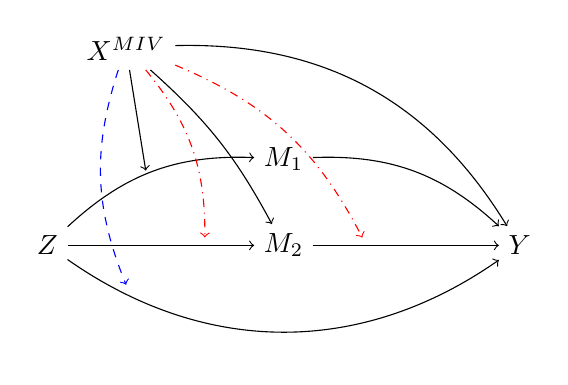
\begin{tikzpicture}
\node at (0,0) (z) {$Z$};
\node at (3,1.1) (m) {$M_1$};
\node at (3,0) (m2) {$M_2$};
\node at (6, 0) (y) {$Y$};
\node at (1,2.5) (x1) {$X^{MIV}$};
\draw[->] 
    (z) edge [bend left = 22.5] (m)
    (m) edge [bend left = 22.5] (y)
    (z) edge [bend right = 35] (y);
\draw[->, dashed, color = blue]
    (x1) edge [bend right = 20] (1, -.5);
\draw[->, dash dot, color = red]
    (x1) edge [bend left = 20] (2, 0.1);
\draw[->, dash dot, color = red]
    (x1) edge [bend left = 20] (4, 0.1);

\draw[->] 
    (x1) edge [bend left = 30] (y);
\draw[->] 
    (x1) edge [bend left = 10] (m2);
\draw[->] (x1)--(1.25, .95);
\draw[->] (z)--(m2);
\draw[->] (m2)--(y);
\end{tikzpicture}

\end{document}